\section{Arbeitspaket 3.1}

\begin{frame}{Topology Discovery and Dynamic Resource Tracking}
    \begin{itemize}
        \item Erfassen der Ressourcen, die auf dem HPC-System zur Verf\"{u}gung
            stehen.
        \item Bereitstellen einer \emph{System-Map} aller Compute-Nodes und
            Speicherkomponenten \emph{(statische Komponente)}.
        \item Darstellung dynamisch genutzter (geteilter) Ressourcen von parallelen
            Anwendungen \emph{(dynamische Komponente)}.
    \end{itemize}
    \begin{block}{Ziel:}
        Die Differenz aus der \emph{System-Map} und der dynamischer Ressourcen-Auslastung
        sind die Ressourcen, die tats\"{a}chlich zur Verf\"{u}gung stehen.
    \end{block}
\end{frame}

\subsection{Topology Discovery}

\begin{frame}{System-Map}
    \begin{block}{System-Map}
        Die System-Map soll einen \"{U}berblick \"{u}ber die HPC-Plattform
        und die zur Verf\"{u}gung stehenden Ressourcen der Plattform bieten.
    \end{block}
    \begin{itemize}
        \item Compute-Nodes mit Anzahl der Cores.
        \item Verf\"{u}gbarer Arbeitsspeicher pro Knoten.
        \item Verf\"{u}gbarer lokaler Speicher (HDD, SSD, NVRAM).
        \item Zentrales Dateisystem mit verf\"{u}gbaren Netzbandbreiten.
        \item Bandbreite zwischen den Compute-Nodes.
    \end{itemize}
\end{frame}

\begin{frame}{Umsetzung via SLURM}
    Umfangreiche Plugin-Architektur z.\,B.\,:
    \begin{itemize}
        \item Topology-Plugins % TODO: links!
        \item Node-Selection-Plugins
    \end{itemize}
    Slurm speichert die Topologie in einer Datei /etc/slurm/topology.conf.\\
    Bietet Informationen zu:
    \begin{itemize}
        \item Anzahl Compute-Nodes
        \item Anzahl Switches
        \item Verbindung zwischen Switches und Compute-Nodes
    \end{itemize}
    \begin{block}{\href{http://slurm.schedmd.com/topology.html}{Topology Guide}}
        At some point in the future Slurm code may be provided to gather network
        topology information directly. Now the network topology information must be
        included in a topology.conf configuration file\ldots
    \end{block}
    \tiny{\footnote{http://slurm.schedmd.com}}
\end{frame}


\begin{frame}{hwloc - The portable Hardware Locality}

    Open-MPI Projekt: Bibliothek und Tools.\\
    Umfasst CLI und C-API.

    \begin{itemize}
    \item Sammelt alle verf\"{u}gbaren Informationen vom OS.
    \item Erstellt abstrakten Baum von Objekten z.B.\,: memory nodes, caches,
        processors, sockets, processor cores, \ldots
    \item Lokalit\"{a}t von I/O devices z.B.\,: network interfaces, Infiniband HCAs
        oder GPUs.
    \item PCI Ger\"{a}te Erkennung z.B.\,: OpenCL, CUDA und Xeon Phi
        Beschleuniger.
    \end{itemize}


    In vielen Projekten bereits genutzt.\\
    \begin{itemize}
        \item PaRSEC
        \item StarPU
        \item TORQUE - resource manager
        \item likwid
    \end{itemize}

    %The hwloc core gathers all the available pieces of information from the
    %operating system and builds an abstracted, portable tree of objects: memory
    %nodes (and node groups), caches, processor sockets, processor cores,
    %hardware threads, and so on.

    %The entire tree of objects is presented in a cross-linked data structure; the
    %tree can be traversed via children, parents, siblings, and cousins.

    %It also gathers various system attributes such as cache and memory
    %information as well as the locality of I/O devices such as network
    %interfaces, InfiniBand HCAs or GPUs.

    %Additionally hwloc can detect the locality PCI devices as well as OpenCL,
    %CUDA and Xeon Phi accelerators, network and InfiniBand interfaces, etc.

\end{frame}


\begin{frame}{hwloc - The portable Hardware Locality}

    \begin{figure}
        \centering
        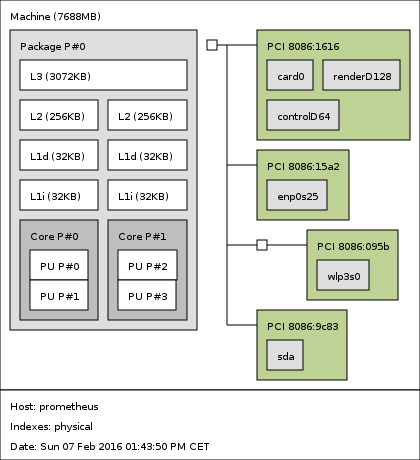
\includegraphics[width=0.58\textwidth]{fig/prometheus.png}
    \end{figure}
\end{frame}


\begin{frame}{netloc - Network Locality}

    Open-MPI Projekt.\\
    Erm\"{o}glicht Informationen \"{u}ber die Netzwerktopologie von HPC-Clustern zu identifizieren.
    \begin{itemize}
        \item Abstrakte Representation als Graph.
        \item Unterst\"{u}tzung f\"{u}r Ethernet und Infiniband Netzwerke.
        \item In Kombination mit \emph{hwloc} umfassende Sicht der Komponenten
            verschiedener Knoten und dem dazwischen liegendem Netzwerk.
    \end{itemize}

    %Additionally, by combining the hwloc single-server topology data with the
    %network topology data, netloc provides developers with a comprehensive view
    %of the HPC system topology, spanning from the processor cores in one server
    %all the way to the cores in another – including the complex network(s) in
    %between.

    %This first public release of the netloc project includes support for
    %OpenFlow-managed Ethernet and InfiniBand networks

\end{frame}


\begin{frame}{netloc - Network Locality}
    \begin{figure}
        \centering
        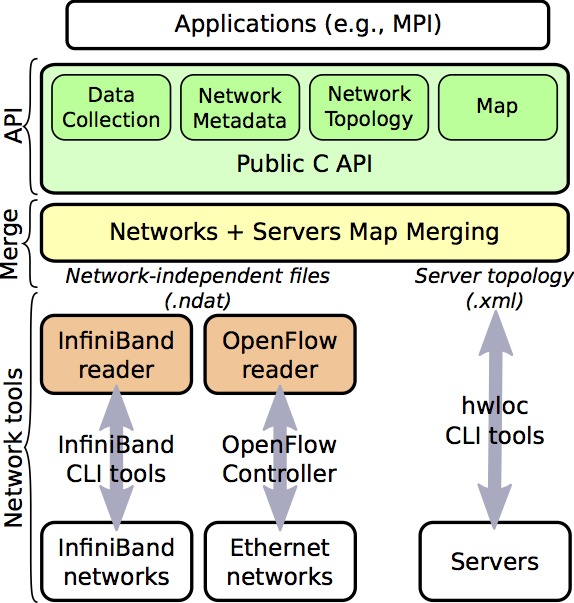
\includegraphics[width=0.58\textwidth]{fig/netloc-design.png}
    \end{figure}
    \tiny{\href{netloc}{https://www.open-mpi.org/projects/netloc/netloc-design-full-size.png}}
\end{frame}


%Starting with hwloc 2.0, both netloc and hwloc are distributed in hwloc releases.

\begin{frame}{Vorschlag}
    \begin{itemize}
        \item Entwicklung eines Tools auf Basis von hwloc und netloc zum
            identifizieren der Topologie.
        \item Einfaches Interface zum Abfragen der Informationen (einfach integrierbar).
        \item Unterst\"{u}tzung mehrerer Ausgabeformate z.B. als OTF2
            Stystem-Tree.
    \end{itemize}
    %(output als OTF2 System-Tree)
\end{frame}
